\documentclass[12pt]{article}%[final]
\setcounter{secnumdepth}{3}
% if you need to pass options to natbib, use, e.g.:
% \PassOptionsToPackage{numbers, compress}{natbib}
% before loading nips_2016
%
% to avoid loading the natbib package, add option nonatbib:
% \usepackage[nonatbib]{nips_2016}

%\usepackage{nips_2016}

% to compile a camera-ready version, add the [final] option, e.g.:
%\usepackage[final]{nips_2016}
\usepackage{amsmath}
\usepackage[utf8]{inputenc} % allow utf-8 input
\usepackage[T1]{fontenc}    % use 8-bit T1 fonts
\usepackage{hyperref}       % hyperlinks
\hypersetup{
     colorlinks   = true,
     citecolor    = black,
     linkcolor    = black
}
\usepackage{url}            % simple URL typesetting
\usepackage{booktabs}       % professional-quality tables
\usepackage{amsfonts}       % blackboard math symbols
\usepackage{nicefrac}       % compact symbols for 1/2, etc.
\usepackage{microtype}      % microtypography
\usepackage{float}
\usepackage{amssymb}
\usepackage{amsthm}
\usepackage{color,soul}
\usepackage{amsmath}
\usepackage{algorithm}
\usepackage[noend]{algpseudocode}
\usepackage[margin=1.5in]{geometry}
\usepackage[english]{babel}
\usepackage{graphicx}
\usepackage{longtable}
\usepackage{verbatim}
\usepackage{setspace}
\usepackage{subcaption}
\doublespacing

\newtheorem{theorem}{Theorem}[section]
\newtheorem{lemma}[theorem]{Lemma}
\newtheorem{proposition}[theorem]{Proposition}
\newtheorem{corollary}[theorem]{Corollary}
\theoremstyle{definition}
\newtheorem{definition}{Definition}[section]

% Code defs from jss
\newcommand\code{\@codex}
\def\@codex#1{{\normalfont\ttfamily\hyphenchar\font=-1 #1}}
%%\let\code=\texttt
\let\proglang=\textsf
\newcommand{\pkg}[1]{{\fontseries{b}\selectfont #1}}


%\theoremstyle{definition}
%\newtheorem{definition}{Definition}[section]


\makeatletter
\def\BState{\State\hskip-\ALG@thistlm}
\makeatother

\title{Time Series Methods in the R package \pkg{mlr}}

% The \author macro works with any number of authors. There are two
% commands used to separate the names and addresses of multiple
% authors: \And and \AND.
%
% Using \And between authors leaves it to LaTeX to determine where to
% break the lines. Using \AND forces a line break at that point. So,
% if LaTeX puts 3 of 4 authors names on the first line, and the last
% on the second line, try using \AND instead of \And before the third
% author name.
\singlespacing
\author{
  Steve Bronder \\
  %Quantitative Methods of the Social Sciences\\
  %Columbia University\\
  %New York City, NY 10027 \\
  \texttt{sab2287@columbia.edu} \\
  %% examples of more authors test etst
   %Department of Computer Science \\
   %Columbia University\\
   %New York City, NY 10027 \\
  %% \AND
  %% Coauthor \\
  %% Affiliation \\
  %% Address \\
  %% \texttt{email} \\
  %% \And
  %% Coauthor \\
  %% Affiliation \\
  %% Address \\
  %% \texttt{email} \\
  %% \And
  %% Coauthor \\
  %% Affiliation \\
  %% Address \\
  %% \texttt{email} \\
}
\doublespacing

\begin{document}
%\SweaveOpts{concordance=TRUE}
% \nipsfinalcopy is no longer used

\maketitle

\begin{abstract}
The \pkg{mlr} package is a unified interface for machine learning tasks such as classification, regression, cluster analysis, and survival analysis. \pkg{mlr} handles the data pipeline of preprocessing, resampling, model selection, model tuning, ensembling, and prediction. This paper details new methods for developing time series models in \pkg{mlr}. This extension includes standard and novel tools such as Lambert $W\times F_X$ transform data generating processes, autoregressive data generating schemes for forecasting with machine learning models, fixed and growing window cross-validation, and forecasting models in the context of univariate and multivariate time series. Examples are given to demonstrate the benefits of a unified framework for machine learning and time series.
\end{abstract}


\section{Introduction}
There has been a rapid development in time series methods over the last 25 years~\cite{Hyndman25} whereby time series models have not only become more common, but more complex. The \proglang{R} language~\cite{Rbase} has several task views that list the extensive amount of packages available for forecasting, time series methods, and empirical finance. While the amount of packages is large, the open source nature of \proglang{R} has left users without a standard syntactic framework whereby individual packages will have a sub-culture of style, syntax, and output. This causes users unnecessary burden, forcing them to memorize and interpret each authors unique style. The \pkg{mlr}~\cite{mlr} package, short for Machine Learning in R, is a meta-package which works to give a strong syntactic framework for the modeling pipeline. By automating and standardizing the tools and methodologies in machine learning, \pkg{mlr} reduces error from the user during the modeling process.

This extension to \pkg{mlr} is the first \proglang{R} package, to this authors knowledge, which gives a fully standardized framework for rigorously testing and training forecasting models\footnote{It is important to recognize that packages like \pkg{forecast} and \pkg{BigVAR} have some pieces of the training framework such as windowing cross-validation and tuning of some of the hyperparameters}. While there are some time series methods available in \pkg{caret}~\cite{caret}, development of forecasting models in \pkg{caret} is difficult due to computational constraints and design choices within the package. The highly modular structure of \pkg{mlr} makes it the best option for implementing time series methods and models. This paper will show how using \pkg{mlr}'s strong syntactic structure allows for time series packages such as \pkg{forecast}~\cite{HyndForecast}, \pkg{rugarch}~\cite{rugarch}, and \pkg{BigVAR}~\cite{BigVAR} to use machine learning methodologies such as automated parameter tuning, data preprocessing, model blending, cross-validation, performance evaluation, and parallel processing techniques for increasing model predictive power.

Section~\ref{sec:m4data} describes the time series data used in this paper to showcase how forecasting is performed in \pkg{mlr}. Section~\ref{sec:task} covers how to create and use univariate and multivariate forecasting tasks. Creating, training, updating, and predicting with basic univariate and multivariate forecasting learners are exampled in section~\ref{seq:build} while tuning and resampling strategies for forecasting are in section~\ref{sec:resamp}. Section~\ref{sec:preproc} covers how using $AR(p,d)$ data generating processes allow for machine learning models to be used in the context of forecasting. Lambert $W\times F_X$ data preprocessing is covered in section~\ref{sec:lambert}. Section~\ref{sec:stackfore} demonstrates how univariate and multivariate forecasting learners can be stacked and ensembled with machine learning models.

\section{Forecasting Data}
\label{sec:m4data}

\subsection{Univariate Forecasting Data}
The standard objective in forecasting is, at time period $t$, make predictions of the target variable $y$ for $t+h$ periods into the future. The difference between standard regression tasks and forecasting is that future values of $y$ are mainly predicted by it’s past. This means that forecasting tasks are most suitable when aspects of past patterns will continue on into the future.

Professional forecasters attempt to predict the future of a series based on its past values. Forecasting has applications in a wide range of tasks including forecasting stock prices~\cite{GRANGER19923}, weather patterns~\cite{MurphymeteoForecast}, international conflicts~\cite{Chadefaux01012014}, and earthquakes~\cite{earthquakeYegu}. The univariate forecasting models will be evaluated using a the daily closing price of Apple Stock (aapl). The training data start on December 12th of 1980 and goes until August 19th, 2016 for a total of 9000 observations. The testing period for the forecast will go from August 22, 2016 to October 10th of 2016 for a total of 35 periods.

\singlespacing

\begin{knitrout}
\definecolor{shadecolor}{rgb}{0.969, 0.969, 0.969}\color{fgcolor}\begin{kframe}


{\ttfamily\noindent\bfseries\color{errorcolor}{\#\# Error in eval(expr, envir, enclos): could not find function "{}Quandl.api\_key"{}}}\end{kframe}
\end{knitrout}

\begin{knitrout}
\definecolor{shadecolor}{rgb}{0.969, 0.969, 0.969}\color{fgcolor}\begin{kframe}
\begin{alltt}
\hlkwd{library}\hlstd{(Quandl)}
\hlkwd{library}\hlstd{(xts)}
\hlstd{aapl} \hlkwb{<-} \hlkwd{Quandl}\hlstd{(}\hlstr{"YAHOO/AAPL"}\hlstd{)}
\hlstd{aaplXts} \hlkwb{<-} \hlkwd{xts}\hlstd{(aapl}\hlopt{$}\hlstd{Close,} \hlkwc{order.by} \hlstd{=} \hlkwd{as.POSIXlt}\hlstd{(aapl}\hlopt{$}\hlstd{Date))}
\hlkwd{colnames}\hlstd{(aaplXts)} \hlkwb{<-} \hlstr{"Close"}
\hlstd{aaplXtsTrain} \hlkwb{<-} \hlstd{aaplXts[}\hlnum{1}\hlopt{:}\hlnum{9000}\hlstd{,]}
\hlstd{aaplXtsTest}  \hlkwb{<-} \hlstd{aaplXts[}\hlnum{9001}\hlopt{:}\hlnum{9035}\hlstd{,]}
\end{alltt}
\end{kframe}
\end{knitrout}



\begin{figure}[h!]
\centering
\begin{minipage}{.5\textwidth}
  \centering
  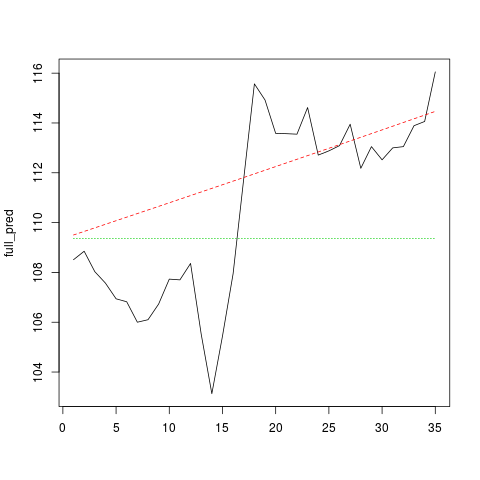
\includegraphics[width=\linewidth]{paper_figures/plot_aapl_train.png}
  \label{fig:aapl_train}
\end{minipage}%
\begin{minipage}{.5\textwidth}
  \centering
  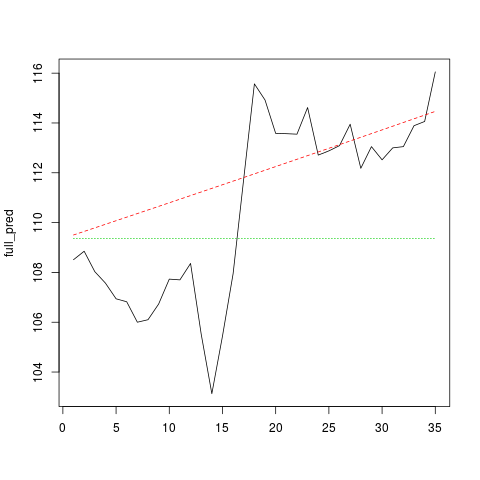
\includegraphics[width=\linewidth]{paper_figures/plot_aapl_test.png}
  \label{fig:aapl_test}
\end{minipage}
\caption{The training and testing data for the univariate models}
\end{figure}

The series is quite complex, with spikes, drops, and many other characteristics of non-stationary time series. This will give the models in mlr a strong test as to what can and cannot be done.

\subsection{Multivariate Forecasting Data}
This paper uses the EUStockMarkets data set from the \pkg{datasets}~\cite{datasets} package to showcase the multivariate forecasting tools. It contains a subset of daily DAX, SMI, CAC, and FTSE European stock indices from July 1st, 1991 to August 24th, 1998 totaling 1828 training observations and 32 test observations.

\singlespace
\begin{knitrout}
\definecolor{shadecolor}{rgb}{0.969, 0.969, 0.969}\color{fgcolor}\begin{kframe}
\begin{alltt}
\hlcom{# Read in Stock Market Data}
\hlkwd{data}\hlstd{(}\hlstr{"EuStockMarkets"}\hlstd{)}
\hlstd{EuStockMarkets.time} \hlkwb{=} \hlstd{lubridate}\hlopt{::}\hlkwd{date_decimal}\hlstd{(}
                \hlkwd{as.numeric}\hlstd{(}\hlkwd{time}\hlstd{(EuStockMarkets)))}
\hlstd{EuStockMarkets}  \hlkwb{=} \hlstd{xts}\hlopt{::}\hlkwd{xts}\hlstd{(}\hlkwd{as.data.frame}\hlstd{(EuStockMarkets),}
                           \hlkwc{order.by} \hlstd{= EuStockMarkets.time)}
\hlstd{eu.train} \hlkwb{=} \hlstd{EuStockMarkets[}\hlnum{1}\hlopt{:}\hlnum{1828}\hlstd{,]}
\hlstd{eu.test} \hlkwb{=} \hlstd{EuStockMarkets[}\hlnum{1829}\hlopt{:}\hlnum{1860}\hlstd{,]}
\end{alltt}
\end{kframe}
\end{knitrout}



\doublespacing

Figure~\ref{fig:eu_train} shows the plot of each series. Note that each stock index tends to follow a similar, but diverging, trend. This will be important to note when performing windowed cross-validation as it will be a real test to see how well the models adapt to what appears to be nonstationary data.

\begin{figure}[h!]
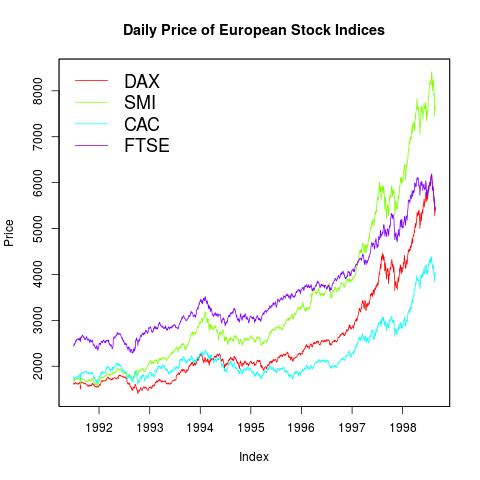
\includegraphics[width=\linewidth]{paper_figures/plot_eu_train.png}
\centering
\caption{The training data from the EuStockMarkets dataset}
\label{fig:eu_train}
\end{figure}

\section{Univariate and Multivariate Forecasting Tasks}
\label{sec:task}

\subsection{Univariate Tasks}
\label{sec:univarTask}
\pkg{mlr} uses the S3 object system to clearly define a predictive modeling task. Tasks contain the data and other relevant meta-information such as the task id and for supervised learning problems the target variable. Forecasting tasks are handled in \pkg{mlr} by the function \code{makeForecastRegrTask()}. The forecasting task inherets most of it's arguments from \code{makeRegrTask}, but has two additional arguments.

\begin{itemize}
\item[data:] Instead of a data frame, an xts object from \pkg{xts}~\cite{xts} containing the time series.
\item[frequency:] An integer representing the periodicity of the time series. For example, daily data with a weekly periodicity has a frequency of 7, daily data with a yearly periodicity has a frequency of 365, and weekly data with a yearly frequency has a periodicity of 52.
\end{itemize}

\singlespacing
\begin{knitrout}
\definecolor{shadecolor}{rgb}{0.969, 0.969, 0.969}\color{fgcolor}\begin{kframe}
\begin{alltt}
\hlkwd{library}\hlstd{(mlr)}
\hlstd{aapl.task} \hlkwb{<-} \hlkwd{makeForecastRegrTask}\hlstd{(}
  \hlkwc{id} \hlstd{=} \hlstr{"Forecast aapl Closing Price"}\hlstd{,}
  \hlkwc{data} \hlstd{= aaplXtsTrain,}
  \hlkwc{target}  \hlstd{=} \hlstr{"Close"}\hlstd{,}
  \hlkwc{frequency} \hlstd{=} \hlnum{5L}\hlstd{)}
\hlstd{aapl.task}
\end{alltt}
\begin{verbatim}
## Task: Forecast aapl Closing Price
## Type: fcregr
## Target: Close
## Observations: 9000
## Dates:
##  Start: 1980-12-12 
##  End:   2016-08-19
## Frequency: 5
## Features:
## numerics  factors  ordered 
##        0        0        0 
## Missings: FALSE
## Has weights: FALSE
## Has blocking: FALSE
\end{verbatim}
\end{kframe}
\end{knitrout}
\doublespacing
Like a regression task, this records the type of the learning problem and basic information about the data set such as the start and end dates, frequency, and whether there are missing values. Note that there are zero features in the task because there is only a target variable, which the model itself will use to build features.

\subsection{Multivariate Tasks}
\label{sec:multivarTask}

One common problem with forecasting is that it is hard to use additional explanatory variables or forecast multiple targets that are dependent on one another. If a model with exogenous variables is at time $t$ and is designed to predict ten periods in the future, it needs to know the values of the exogenous variables at time $t+10$, which is often not possible. A new set of models~\cite{BigVAR} which treats exogenous variables endogenously allows forecasters to not only forecast the target, but additional explanatory variables. Forecasting exogenous variables works by treating all the variables as targets, making them endogenous to the model. A multivariate forecasting task is created to hold the data and meta-information for the model. The function \code{makeMultiForecastRegrTask()} has the same arguments as \code{makeForecastRegrTask()} with one exception. The \code{target} argument can contain either a single target variable, multiple target variables, or \code{All} which treats all variables endogenously.

\singlespacing
\begin{knitrout}
\definecolor{shadecolor}{rgb}{0.969, 0.969, 0.969}\color{fgcolor}\begin{kframe}
\begin{alltt}
\hlstd{mfcregr.univar.task} \hlkwb{=} \hlkwd{makeMultiForecastRegrTask}\hlstd{(}\hlkwc{id} \hlstd{=} \hlstr{"bigvar"}\hlstd{,}
                                         \hlkwc{data} \hlstd{= eu.train,}
                                         \hlkwc{target} \hlstd{=} \hlstr{"FTSE"}\hlstd{,}
                                         \hlkwc{frequency} \hlstd{=} \hlnum{5L}\hlstd{)}
\hlstd{mfcregr.univar.task}
\end{alltt}
\begin{verbatim}
## Task: bigvar
## Type: mfcregr
## Target: FTSE
## Observations: 1828
## Dates:
##  Start: 1991-07-01 02:18:27 
##  End:   1998-07-10 22:09:13
## Frequency: 5
## Features:
## numerics  factors  ordered 
##        3        0        0 
## Missings: FALSE
## Has weights: FALSE
## Has blocking: FALSE
\end{verbatim}
\end{kframe}
\end{knitrout}
\doublespacing

Like \code{makeForecastRegrTask()}, \code{mfcregr.univar.task} has the standard output, but notice now that there are three features. Alternatively, \code{mfcregr.all.task} contains multiple target values with no features. The difference between each of these multivariate tasks is that \code{mfcregr.univar.task} will act similar to \code{makeForecastRegrTask()}, giving a univariate forecast output and evaluating the forecasts with univariate measures. When the target is \code{All} or multiple variables the trained model will forecast and output all series and use a multivariate form of the univariate measures. Though the results appear different, both of these tasks will still forecast all of the underlying series, which allows the model take in exogenous variables and treat them endogenously for n-step ahead forecasts that use additional explanatory variables.

\singlespacing
\begin{knitrout}
\definecolor{shadecolor}{rgb}{0.969, 0.969, 0.969}\color{fgcolor}\begin{kframe}
\begin{alltt}
\hlstd{mfcregr.all.task} \hlkwb{=} \hlkwd{makeMultiForecastRegrTask}\hlstd{(}\hlkwc{id} \hlstd{=} \hlstr{"bigvar"}\hlstd{,}
                                      \hlkwc{data} \hlstd{= eu.train,}
                                      \hlkwc{target} \hlstd{=} \hlstr{"all"}\hlstd{,}
                                      \hlkwc{frequency} \hlstd{=} \hlnum{5L}\hlstd{)}
\hlstd{mfcregr.all.task}
\end{alltt}
\begin{verbatim}
## Task: bigvar
## Type: mfcregr
## Target: DAX SMI CAC FTSE
## Observations: 1828
## Dates:
##  Start: 1991-07-01 02:18:27 
##  End:   1998-07-10 22:09:13
## Frequency: 5
## Features:
## numerics  factors  ordered 
##        0        0        0 
## Missings: FALSE
## Has weights: FALSE
## Has blocking: FALSE
\end{verbatim}
\end{kframe}
\end{knitrout}
\doublespacing

\section{Building a forecast learner}
\label{seq:build}
\subsection{Univariate Forecasting}
\label{seq:buildAndTuneUni}

The \code{makeLearner()} function provides a structured model building framework to the several forecasting models currently implemented in \pkg{mlr}. This section will build an exponential smoothing state space model (ETS)~\cite{etsMod} to show how to create forecasting models in \pkg{mlr}.

ETS is one of the most popular forecasting models and is available in \pkg{mlr} along with models such as BATS, ARIMA, TBATS, several GARCH variants, and autoregressive neural networks. Section~\ref{sec:preprocAR} uses preprocessing features to develop arbitrary supervised machine learning models in the context of forecasting. An ETS model is created by calling the function \code{makeLearner()}, supplying the class of learner, the number of steps to forecast, and any additional arguments to be passed to \code{ets()} from \pkg{forecast}.

%\footnote{Possible arguments to the model can be found by using \code{getLearnerParamSet("fcregr.tbats")}.}
\singlespacing
\begin{knitrout}
\definecolor{shadecolor}{rgb}{0.969, 0.969, 0.969}\color{fgcolor}\begin{kframe}
\begin{alltt}
\hlstd{ets.mod} \hlkwb{=}\hlkwd{makeLearner}\hlstd{(}\hlkwc{cl} \hlstd{=} \hlstr{"fcregr.ets"}\hlstd{,} \hlkwc{model} \hlstd{=} \hlstr{"AZA"}\hlstd{,}
                     \hlkwc{h} \hlstd{=} \hlnum{35}\hlstd{,} \hlkwc{predict.type} \hlstd{=} \hlstr{"response"}\hlstd{)}
\hlstd{ets.mod}
\end{alltt}
\begin{verbatim}
## Learner fcregr.ets from package forecast
## Type: fcregr
## Name: Exponential smoothing state space model; Short name: ets
## Class: fcregr.ets
## Properties: numerics,quantile
## Predict-Type: response
## Hyperparameters: model=AZA,h=35
\end{verbatim}
\end{kframe}
\end{knitrout}
\doublespacing

The \code{predict.type} for forecasting models can either be a point estimate (\code{response}) or point estimates with quantiles of confidence intervals (\code{quantile}). The function \code{train()} is called, supplying both the learner and task to build the final model over the full data set.

\singlespace
\begin{knitrout}
\definecolor{shadecolor}{rgb}{0.969, 0.969, 0.969}\color{fgcolor}\begin{kframe}
\begin{alltt}
\hlstd{train.ets} \hlkwb{=} \hlkwd{train}\hlstd{(}\hlkwc{learner} \hlstd{= ets.mod,} \hlkwc{task} \hlstd{= aapl.task )}
\hlstd{train.ets}
\end{alltt}
\begin{verbatim}
## Model for learner.id=fcregr.ets; learner.class=fcregr.ets
## Trained on: task.id = Forecast aapl Closing Price; obs = 9000; features = 0
## Hyperparameters: model=AZA,h=35
\end{verbatim}
\end{kframe}
\end{knitrout}
\doublespace

The forecasts are generated by calling \code{predict()}. Optionally, supplying the test data as an additional argument will allow \pkg{mlr} to return an object containing meta information for the forecasts along with the prediction and test data in columns \code{truth} and \code{response}, respectively.

\singlespacing
\begin{knitrout}
\definecolor{shadecolor}{rgb}{0.969, 0.969, 0.969}\color{fgcolor}\begin{kframe}
\begin{alltt}
\hlstd{predict.ets} \hlkwb{=} \hlkwd{predict}\hlstd{(train.ets,} \hlkwc{newdata} \hlstd{= aaplXtsTest)}
\hlstd{predict.ets}
\end{alltt}
\begin{verbatim}
## Prediction: 35 observations
## predict.type: response
## threshold: 
## time: 0.00
##             truth response
## 2016-08-22 108.51 109.6713
## 2016-08-23 108.85 109.7299
## 2016-08-24 108.03 109.9426
## 2016-08-25 107.57 109.7255
## 2016-08-26 106.94 109.3600
## 2016-08-29 106.82 109.6713
## ... (35 rows, 2 cols)
\end{verbatim}
\end{kframe}
\end{knitrout}
\doublespacing

The model is evaluated by calling \code{performance()} with the Mean Absolute Scaled Error (MASE)~\cite{Hyndman2006} measure.

\singlespacing
\begin{knitrout}
\definecolor{shadecolor}{rgb}{0.969, 0.969, 0.969}\color{fgcolor}\begin{kframe}
\begin{alltt}
\hlkwd{performance}\hlstd{(predict.ets,} \hlkwc{measure} \hlstd{= mase,}
            \hlkwc{task} \hlstd{= aapl.task)}
\end{alltt}
\begin{verbatim}
##      mase 
## 0.8073069
\end{verbatim}
\end{kframe}
\end{knitrout}
\doublespacing
MASE has favorable properties for calculating forecast errors relative to measures such as root mean squared error or median relative absolute error. Arguably one of the most important features, it is very interpretable. Let $y_t$ and $\tilde{y}_t$ be the target variable and prediction at time $t$ with $\epsilon_t = y_t - \tilde{y}_t$ being the forecast error. Then MASE is calculated as

\begin{equation}
\text{MASE} = \frac{\sum_{t=1}^T |\epsilon_t|}{\frac{T}{T-1} \sum_{t=2}^T |y_{t, \text{insample}} - y_{t-1, \text{insample}}|}
\end{equation}

Where the denominator is the one step ahead naive forecast from the training data. When the numerator is equal to the denominator, the model performs as well as a simple naive forecast method. A MASE score greater than one indicates the model is performing worse than the naive forecasting method while scores less than one mean the model is performing better than the naive forecasting method.

The scale invariance of MASE means that it is independent of the scale of the data and allows model comparison across data sets. The scale invariance of MASE has made it a favorite for comparing the accuracy of forecast methods~\cite{noteMase} across datasets. While scaling in measures such as the Mean Absolute Percentage Error can cause poor behavior as the target variable goes to zero, MASE does not become skewed when the target variable approaches zero. Having good properties near zero allows the use of MASE in situations in which zeros occur frequently or zero is not meaningful such as predicting temperature. The model does a successful job of catching the downward trend, but figure~\ref{fig:ets_train} shows the downward bias of the model which does not allow it to account for the sharp upward swings.

\singlespacing


\doublespacing

\begin{figure}[h!]
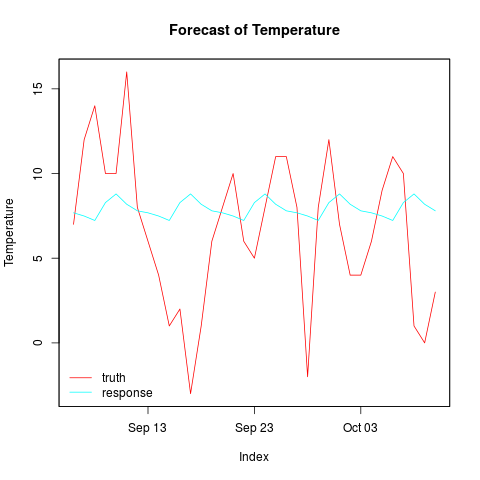
\includegraphics[width=\linewidth]{paper_figures/plot_ets_train.png}
\centering
\caption{The forecasts response from ets against the testing data}
\label{fig:ets_train}
\end{figure}

\subsection{Updating Forecast Models}

 Forecasting models are designed to predict the next $n$ values that will appear in the series. Without a way to update the model with new data, the model will have to be completely rebuilt for each new set of forecasts. The \code{updateModel} function allows forecasters to avoid the expensive cost of retraining the entire forecasting model. The function updates the model with new points which then allows for updated forecasts.

\singlespacing
\begin{knitrout}
\definecolor{shadecolor}{rgb}{0.969, 0.969, 0.969}\color{fgcolor}\begin{kframe}
\begin{alltt}
\hlstd{update.ets} \hlkwb{=} \hlkwd{updateModel}\hlstd{(train.ets, aapl.task,}
                           \hlkwc{newdata} \hlstd{= aaplXtsTest)}
\hlkwd{predict}\hlstd{(update.ets,} \hlkwc{task} \hlstd{= aapl.task)}
\end{alltt}
\begin{verbatim}
## Prediction: 35 observations
## predict.type: response
## threshold: 
## time: 0.00
##                     response
## 2016-08-20 10:45:39 116.2968
## 2016-08-21 21:31:19 116.7730
## 2016-08-23 08:16:59 116.6052
## 2016-08-24 19:02:39 115.8487
## 2016-08-26 05:48:19 116.0500
## 2016-08-27 16:33:59 116.2968
## ... (35 rows, 1 cols)
\end{verbatim}
\end{kframe}
\end{knitrout}
\doublespacing

All univariate forecasting models have access to the \code{updateModel()} function. Future versions of \code{mlr} will also include online machine learning models that can be updated as new data comes in.

\subsection{Multivariate Forecasting}
\label{seq:buildAndTuneMulti}

Multivariate forecasting in \pkg{mlr} uses the package \pkg{BigVAR}~\cite{bigvarpaper}. \pkg{BigVAR} allows for estimation of high dimensional time series through methods such as structured Lasso penalties to find the optimal autoregressive structures through cross-sections and time.

\singlespacing
\begin{knitrout}
\definecolor{shadecolor}{rgb}{0.969, 0.969, 0.969}\color{fgcolor}\begin{kframe}
\begin{alltt}
\hlstd{bigvar.mod} \hlkwb{=} \hlkwd{makeLearner}\hlstd{(}\hlstr{"mfcregr.BigVAR"}\hlstd{,}\hlkwc{p} \hlstd{=} \hlnum{25}\hlstd{,}
                         \hlkwc{struct} \hlstd{=} \hlstr{"SparseLag"}\hlstd{,}
                         \hlkwc{gran} \hlstd{=} \hlkwd{c}\hlstd{(}\hlnum{50}\hlstd{,} \hlnum{60}\hlstd{),}\hlkwc{h} \hlstd{=} \hlnum{35}\hlstd{,} \hlkwc{n.ahead} \hlstd{=} \hlnum{35}\hlstd{)}
\end{alltt}
\end{kframe}
\end{knitrout}
\doublespacing

This section uses the multivariate forecast task which has all variables as targets, while section~\ref{sub:multiStack} performs the single target multivariate forecast with a stacked predictor. Multiforecast regressions operate the same as other supervised models, supplying a task and learner to \code{train()}.

\singlespacing
\begin{knitrout}
\definecolor{shadecolor}{rgb}{0.969, 0.969, 0.969}\color{fgcolor}\begin{kframe}
\begin{alltt}
\hlstd{train.bigvar} \hlkwb{=} \hlkwd{train}\hlstd{(}\hlkwc{learner} \hlstd{= bigvar.mod,}
                     \hlkwc{task} \hlstd{= mfcregr.all.task )}
\hlstd{train.bigvar}
\end{alltt}
\end{kframe}
\end{knitrout}

\begin{knitrout}
\definecolor{shadecolor}{rgb}{0.969, 0.969, 0.969}\color{fgcolor}\begin{kframe}
\begin{verbatim}
## Model for learner.id=mfcregr.BigVAR; learner.class=mfcregr.BigVAR
## Trained on: task.id = bigvar; obs = 1828; features = 0
## Hyperparameters: p=25,struct=SparseLag,gran=50,60,h=35,n.ahead=35
\end{verbatim}
\end{kframe}
\end{knitrout}
\doublespacing

Predictions for \code{multiForecast} methods have a similar output to \code{multiclass} methods, returning multiple truth and response variables. For multivariate forecasts, a multivariate version of MASE takes the mean of each MASE score for the individual variables as the performance measure.

\begin{equation}
\text{MultiMASE} = \frac{\sum_{i=1}^m \text{MASE}_i}{m}
\end{equation}

given that $m$ is the number of variables that are forecast.

\singlespacing
\begin{knitrout}
\definecolor{shadecolor}{rgb}{0.969, 0.969, 0.969}\color{fgcolor}\begin{kframe}
\begin{alltt}
\hlstd{predict.bigvar} \hlkwb{=} \hlkwd{predict}\hlstd{(train.bigvar,} \hlkwc{newdata} \hlstd{= eu.test)}
\hlstd{predict.bigvar}
\end{alltt}
\begin{verbatim}
## Prediction: 32 observations
## predict.type: response
## threshold: 
## time: 0.02
##                     truth.DAX truth.SMI truth.CAC truth.FTSE response.DAX
## 1998-07-12 07:50:46   5905.15    8047.3    4252.1     5960.2     5852.841
## 1998-07-13 17:32:18   5961.45    8099.0    4304.4     5988.4     5820.194
## 1998-07-15 03:13:50   5942.06    8166.0    4311.1     5990.3     5801.712
## 1998-07-16 12:55:23   5975.88    8160.0    4333.1     6003.4     5790.565
## 1998-07-17 22:36:55   6018.89    8227.2    4339.9     6009.6     5781.540
## 1998-07-19 08:18:27   6000.84    8205.0    4319.2     5969.7     5772.087
##                     response.SMI response.CAC response.FTSE
## 1998-07-12 07:50:46     7982.503     4192.149      5997.825
## 1998-07-13 17:32:18     7960.779     4153.550      6037.958
## 1998-07-15 03:13:50     7955.264     4130.674      6063.687
## 1998-07-16 12:55:23     7958.119     4115.612      6083.094
## 1998-07-17 22:36:55     7965.061     4103.302      6100.075
## 1998-07-19 08:18:27     7973.586     4091.154      6116.419
## ... (32 rows, 8 cols)
\end{verbatim}
\begin{alltt}
\hlkwd{performance}\hlstd{(predict.bigvar, multivar.mase,}
            \hlkwc{task} \hlstd{= mfcregr.all.task)}
\end{alltt}
\begin{verbatim}
## multivar.mase 
##       12.7678
\end{verbatim}
\end{kframe}
\end{knitrout}


\begin{figure}[H]
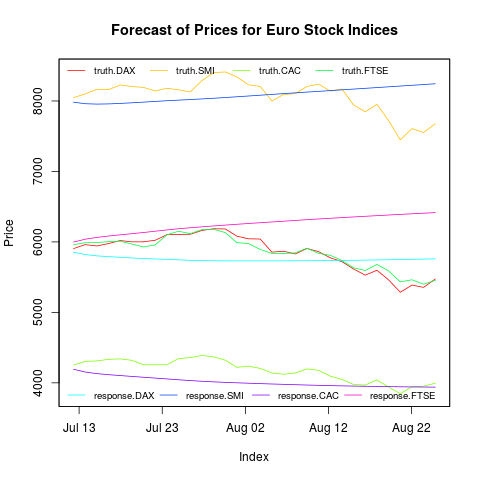
\includegraphics[width=.8\linewidth]{paper_figures/plot_bigvar_train.png}
\centering
\caption{The forecasts response from BigVAR against the true test stock index data}
\label{fig:bigvar_train}
\end{figure}
\doublespacing

\section{Resampling with Time}
\label{sec:resamp}


While ETS is one of the most popular time series models the error type, trend type, season type, and whether to include a damped or multiplicative trend can be a subjective process that will almost always lead to a sub-optimal model selection. One of the first proposals for automated forecasting methods comes from~\cite{hannanOrder} for automatic order selection of ARIMA models. Innovations are obtained by fitting high order autoregressive models to the data and then computing the likelihood of potential models through a series of standard regression. Proprietary algorithms from software such as \proglang{Forecast Pro}~\cite{forecastpro} and \proglang{Autobox}~\cite{reillyautobox} are well known and have performed to high standards in competitions such as the M3 forecasting competition~\cite{Makridakis2000451}. One of the most prominent R packages for automated forecasting is \pkg{forecast}~\cite{HyndForecast} which contains several methods for automated forecasting including exponential smoothing based methods and step-wise algorithms for finding optimal ARIMA models.

Forecasting in \pkg{mlr} takes a machine learning approach, creating a parameter set for a given model and using an optimization method to search over the parameter space. The forecasting extension of \pkg{mlr} includes growing and fixed window resampling schemes to train over the possible models. Resampling schemes such as cross-validation and bootstrapping are common in machine learning for dealing with the bias-variance tradeoff~\cite{Friedman1997}~\cite{rodriguezkfold}. When there is a time component to the data, windowing schemes are useful in allowing a valid resampling scheme while still accounting for the time properties of the series. Figure~\ref{fig:caret} gives an example of fixed and growing window cross validation. Let $h$ be a forecast horizon where the index of the starting and end points of the training data are $\text{start}_i$ and $\text{end}_i$ where $i$ is the index for each window. The first model will train on data between $\text{start}_i$ and $\text{end}_i$ while testing on data indexed between $\text{end}_i + h$. After each iteration the window slides forward $h$ steps such that $\text{end}_{i+1} = \text{end}_{i} + h$. In the case of the fixed window, the starting index will also shift such that $\text{start}_{i+1} = \text{start}_{i} + h$ while $\text{start}_i$ will remain constant in the growing window case. This type of growing and fixed window resampling~\cite{hyndman2014forecasting} is now available in the \code{resampling()} function of \pkg{mlr}.

\begin{figure}[h!]
  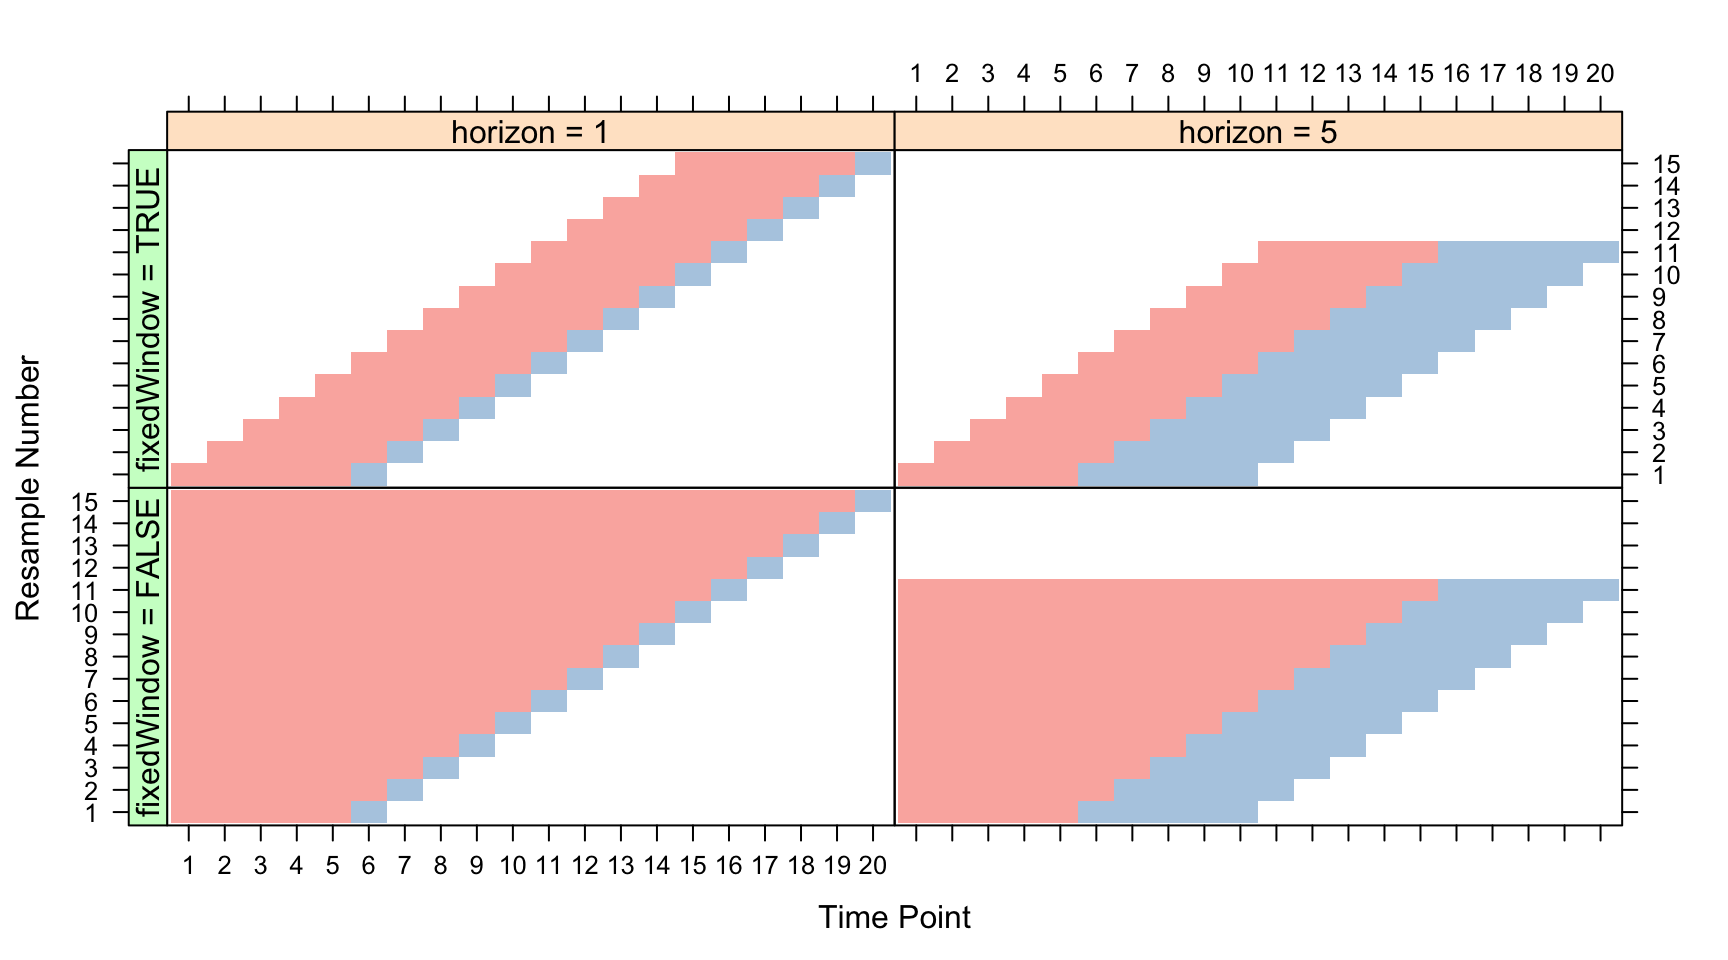
\includegraphics[width=\linewidth]{paper_figures/windowing_pic_caret}
  \centering
  \caption{Resampling with a window scheme as exampled by \pkg{caret}~\cite{windowingcaret}. The top graphs are fixed window cross validation while the bottom graphs are growing window cross validation. }
  \label{fig:caret}
\end{figure}

To create a windowing resampling process, the function \code{makeResampleDesc()} uses the resampling type, the horizon, initial window, the length of the series, and an optional argument to skip over some windows for the sake of time.

\singlespacing
\begin{knitrout}
\definecolor{shadecolor}{rgb}{0.969, 0.969, 0.969}\color{fgcolor}\begin{kframe}
\begin{alltt}
\hlstd{resampDesc} \hlkwb{=} \hlkwd{makeResampleDesc}\hlstd{(}\hlstr{"GrowingCV"}\hlstd{,} \hlkwc{horizon} \hlstd{=} \hlnum{35L}\hlstd{,}
                              \hlkwc{initial.window} \hlstd{=} \hlnum{.4}\hlstd{,}
                              \hlkwc{size} \hlstd{=} \hlkwd{nrow}\hlstd{(}\hlkwd{getTaskData}\hlstd{(aaplTask)),}
                              \hlkwc{skip} \hlstd{=} \hlnum{.03}\hlstd{)}
\end{alltt}


{\ttfamily\noindent\bfseries\color{errorcolor}{\#\# Error in checkClass(x, classes, ordered): object 'aaplTask' not found}}\begin{alltt}
\hlstd{resampDesc}
\end{alltt}


{\ttfamily\noindent\bfseries\color{errorcolor}{\#\# Error in eval(expr, envir, enclos): object 'resampDesc' not found}}\end{kframe}
\end{knitrout}
\doublespacing

The methods in package \pkg{ParamHelpers}~\cite{paramhelper} allow \pkg{mlr} to have a simple and rigorous interface for creating parameter spaces. There are several types of tools to help search the parameter space including grid search, random search~\cite{Bergstra}, iterated F-racing~\cite{irace}, Simulated Annealing, and CMA-ES~\cite{cmaes}  to search the parameter space for the most optimal model. This ETS model uses only discrete and logical parameters, however functions are available for numeric, integer, numeric vectors, and several other types of parameters.


\singlespacing
\begin{knitrout}
\definecolor{shadecolor}{rgb}{0.969, 0.969, 0.969}\color{fgcolor}\begin{kframe}
\begin{alltt}
  \hlkwd{makeDiscreteParam}(\hlstr{"model"}, values = \hlkwd{c}(\hlstr{"ANN"}, \hlstr{"MNN"}, \hlstr{"ZNN"},
                                        \hlstr{"AAN"}, \hlstr{"MAN"}, \hlstr{"ZAN"},
                                        \hlstr{"AMN"}, \hlstr{"MMN"}, \hlstr{"ZMN"},
                                        \hlstr{"AZN"}, \hlstr{"MZN"}, \hlstr{"ZZN"},
                                        \hlstr{"ANA"}, \hlstr{"MNA"}, \hlstr{"ZNA"},
                                        \hlstr{"AAA"}, \hlstr{"MAA"}, \hlstr{"ZAA"},
                                        \hlstr{"AMA"}, \hlstr{"MMA"}, \hlstr{"ZMA"},
                                        \hlstr{"AZA"})),
  \hlkwd{makeLogicalParam}(\hlstr{"damped"}),
  \hlkwd{makeLogicalParam}(\hlstr{"additive.only"}),
  \hlkwd{makeLogicalParam}(\hlstr{"biasadj"}),
  \hlkwd{makeDiscreteParam}(\hlstr{"opt.crit"}, values = \hlkwd{c}(\hlstr{"amse"},
                                           \hlstr{"sigma"}, \hlstr{"mae"},
                                           \hlstr{"lik"})),
  \hlkwd{makeDiscreteParam}(\hlstr{"ic"}, values = \hlkwd{c}(\hlstr{"aicc"}, \hlstr{"aic"}, \hlstr{"bic"})),
  \hlkwd{makeLogicalParam}(\hlstr{"allow.multiplicative.trend"})
)

ctrl = \hlkwd{makeTuneControlIrace}(maxExperiments = 700L)
\end{alltt}
\end{kframe}
\end{knitrout}
\doublespacing

Using \code{tuneParams()}, the model is tuned for the task using the specified resampling scheme, parameter set, tune control, and measure. This tuning task uses MASE~\cite{Hyndman2006} as a measure of performance \footnote{If a frequency is defined in the task, the seasonal MASE score will be used.}. The model is also tuned in parallel using the package \pkg{parallelMap}~\cite{parallel} for it's built in compatibility with \pkg{mlr}.

\singlespacing
\begin{knitrout}
\definecolor{shadecolor}{rgb}{0.969, 0.969, 0.969}\color{fgcolor}\begin{kframe}
\begin{alltt}
\hlkwd{library}\hlstd{(}\hlstr{"parallelMap"}\hlstd{)}
\hlkwd{parallelStart}\hlstd{(}\hlstr{"multicore"}\hlstd{,} \hlnum{7}\hlstd{)}
\hlkwd{configureMlr}\hlstd{(}\hlkwc{on.learner.error} \hlstd{=} \hlstr{"warn"}\hlstd{)}
\hlkwd{set.seed}\hlstd{(}\hlnum{1234}\hlstd{)}
\hlstd{ets.tune.aapl} \hlkwb{=} \hlkwd{tuneParams}\hlstd{(}\hlkwd{makeLearner}\hlstd{(}\hlstr{"fcregr.ets"}\hlstd{,} \hlkwc{h} \hlstd{=} \hlnum{35}\hlstd{),}
                     \hlkwc{task} \hlstd{= aapl.task,}
                     \hlkwc{resampling} \hlstd{= resampDesc,} \hlkwc{par.set} \hlstd{= parSet,}
                     \hlkwc{control} \hlstd{= ctrl,} \hlkwc{measures} \hlstd{= mase)}
\hlkwd{parallelStop}\hlstd{()}
\end{alltt}
\end{kframe}
\end{knitrout}



\begin{knitrout}
\definecolor{shadecolor}{rgb}{0.969, 0.969, 0.969}\color{fgcolor}\begin{kframe}


{\ttfamily\noindent\color{warningcolor}{\#\# Warning in readChar(con, 5L, useBytes = TRUE): cannot open compressed file './models/etsTuneFeb27th.RData', probable reason 'No such file or directory'}}

{\ttfamily\noindent\bfseries\color{errorcolor}{\#\# Error in readChar(con, 5L, useBytes = TRUE): cannot open the connection}}

{\ttfamily\noindent\bfseries\color{errorcolor}{\#\# Error in eval(expr, envir, enclos): object 'ets.tune.aapl' not found}}\end{kframe}
\end{knitrout}

\doublespace

Using \pkg{mlr}'s built in plotting routines the tuning parameters can be analyzed\footnote{Because of constraints which do not allow logical types in the partial dependence plots, the below code takes all of the logical parameters from \code{ets.tune.aapl} and coerces them to be numeric} graphically using partial dependence plots~\cite{partialdep}.

\singlespace

\begin{knitrout}
\definecolor{shadecolor}{rgb}{0.969, 0.969, 0.969}\color{fgcolor}\begin{kframe}
\begin{alltt}
\hlcom{# Make data for dependence plot}
\hlstd{ets.hyp} \hlkwb{=} \hlkwd{generateHyperParsEffectData}\hlstd{(ets.tune.aapl,} \hlkwc{partial.dep} \hlstd{=} \hlnum{TRUE}\hlstd{,}
                                        \hlkwc{trafo} \hlstd{=} \hlnum{TRUE}\hlstd{)}
\end{alltt}


{\ttfamily\noindent\bfseries\color{errorcolor}{\#\# Error in checkClass(tune.result, "{}ResampleResult"{}): object 'ets.tune.aapl' not found}}\end{kframe}
\end{knitrout}

\begin{knitrout}
\definecolor{shadecolor}{rgb}{0.969, 0.969, 0.969}\color{fgcolor}\begin{kframe}


{\ttfamily\noindent\bfseries\color{errorcolor}{\#\# Error in eval(expr, envir, enclos): object 'ets.hyp' not found}}

{\ttfamily\noindent\bfseries\color{errorcolor}{\#\# Error in eval(expr, envir, enclos): object 'ets.hyp' not found}}

{\ttfamily\noindent\bfseries\color{errorcolor}{\#\# Error in eval(expr, envir, enclos): object 'ets.hyp' not found}}

{\ttfamily\noindent\bfseries\color{errorcolor}{\#\# Error in eval(expr, envir, enclos): object 'ets.hyp' not found}}

{\ttfamily\noindent\bfseries\color{errorcolor}{\#\# Error in eval(expr, envir, enclos): object 'ets.hyp' not found}}\end{kframe}
\end{knitrout}

\begin{knitrout}
\definecolor{shadecolor}{rgb}{0.969, 0.969, 0.969}\color{fgcolor}\begin{kframe}
\begin{alltt}
\hlcom{# Making graphics}
\hlkwd{plotHyperParsEffect}\hlstd{(ets.hyp,} \hlkwc{x}\hlstd{=} \hlstr{"model"}\hlstd{,} \hlkwc{y} \hlstd{=} \hlstr{"mase.test.mean"}\hlstd{,}
                     \hlkwc{plot.type} \hlstd{=} \hlstr{"scatter"}\hlstd{,}
                     \hlkwc{partial.dep.learn} \hlstd{=} \hlstr{"regr.randomForest"}\hlstd{)}
\hlkwd{plotHyperParsEffect}\hlstd{(ets.hyp,} \hlkwc{x}\hlstd{=} \hlstr{"opt.crit"}\hlstd{,} \hlkwc{y} \hlstd{=} \hlstr{"mase.test.mean"}\hlstd{,}
                     \hlkwc{plot.type} \hlstd{=} \hlstr{"scatter"}\hlstd{,}
                     \hlkwc{partial.dep.learn} \hlstd{=} \hlstr{"regr.randomForest"}\hlstd{)}
\end{alltt}
\end{kframe}
\end{knitrout}







































































































